\documentclass{article}
\usepackage[margin=1.0in]{geometry}
\usepackage{amsmath, amssymb, mathrsfs}
\usepackage[english]{babel}
\usepackage{graphicx}
\usepackage{enumerate}
\usepackage{listings}
\usepackage{tikz}
\renewcommand{\vec}[1]{\mathbf{#1}}
\newcommand{\floor}[1]{\left\lfloor #1 \right\rfloor}
\newcommand{\ceil}[1]{\left\lceil #1 \right\rceil}

\title{Machine Learning from Data Assignment 12}
\author{Greg Stewart}
\date{\today}

\begin{document}

\maketitle

\subsection*{Neural Networks and Backpropagation.}

\begin{enumerate}[(a)]
  \item \textit{Gradient}

    Identity output node:

    $$G_1 = \begin{pmatrix} -.0322 & -.0322 \\ -.0322 & -.0322 \\ -.0322 & -.0322 \end{pmatrix}
      \qquad
      G_2 = \begin{pmatrix} -.2162 \\ -.1373 \\ -.1373 \end{pmatrix}$$

    And for the tanh() output node:

    $$G_1 = \begin{pmatrix} -.0267 & -.0267 \\ -.0267 & -.0267 \\ -.0267 & -.0267 \end{pmatrix}
      \qquad
      G_2 = \begin{pmatrix} -.1791 \\ -.1137 \\ -.1137 \end{pmatrix}$$

  \item \textit{Perturbation}

    Identity output node:

    $$G_1 = \begin{pmatrix} -.03224 & -.03224 \\ -.03224 & -.03224 \\ -.03224 & -.03224 \end{pmatrix}
      \qquad
      G_2 = \begin{pmatrix} -.2162 \\ -.1373 \\ -.1373 \end{pmatrix}$$

    And for the tanh() output node:

    $$G_1 = \begin{pmatrix} -.0267 & -.0267 \\ -.0267 & -.0267 \\ -.0267 & -.0267 \end{pmatrix}
      \qquad
      G_2 = \begin{pmatrix} -.1790 \\ -.11372 \\ -.11372 \end{pmatrix}$$

        These results are very very close to the gradient results (although not clearly shone,
        they typically differ in the 1e-5 place of the decimal).

\end{enumerate}


\subsection*{Neural Networks for Digits.}

\begin{enumerate}[(a)]
  \item \textit{}

    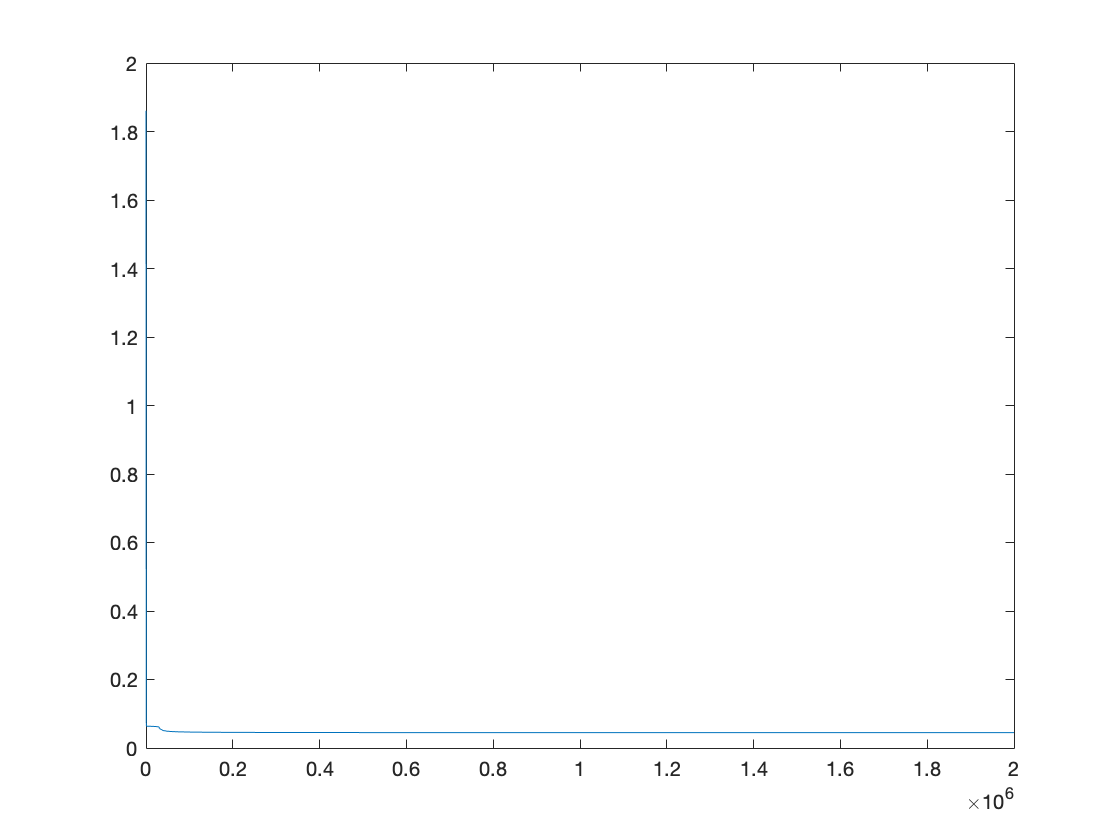
\includegraphics[width=.4\textwidth]{nna1.png}
    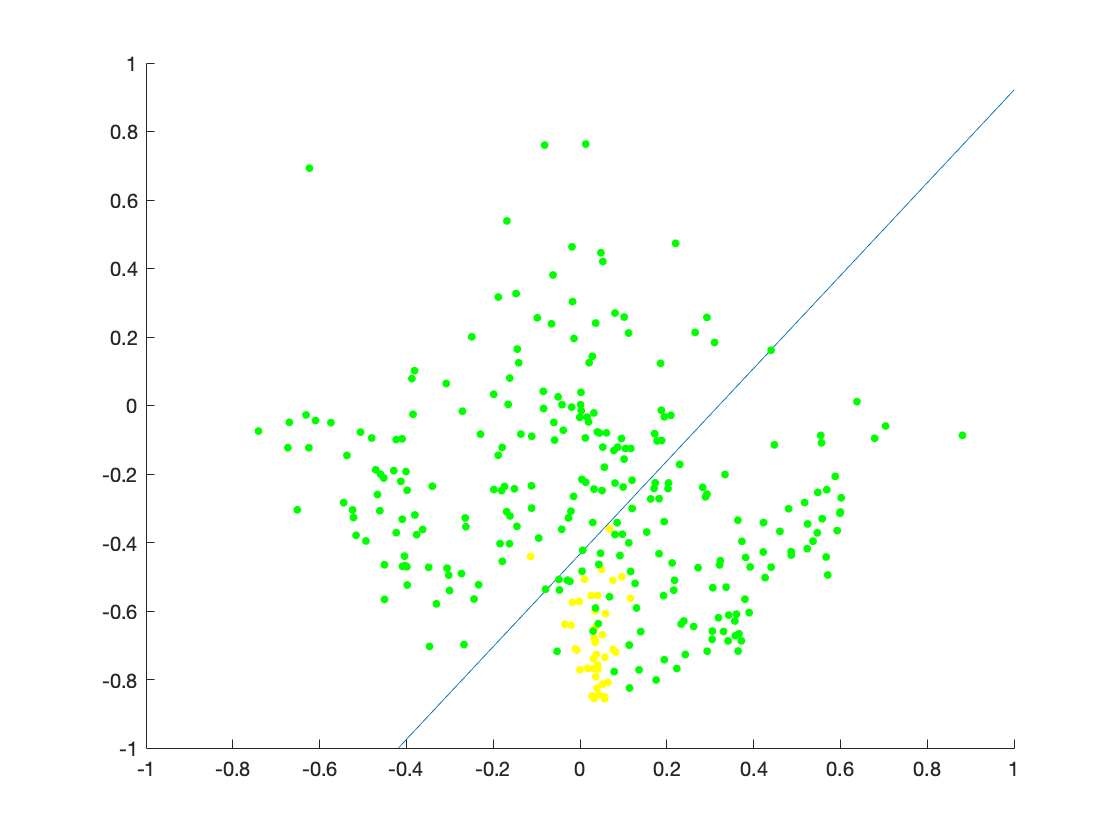
\includegraphics[width=.4\textwidth]{nna1boundary.png}

  \item \textit{}

    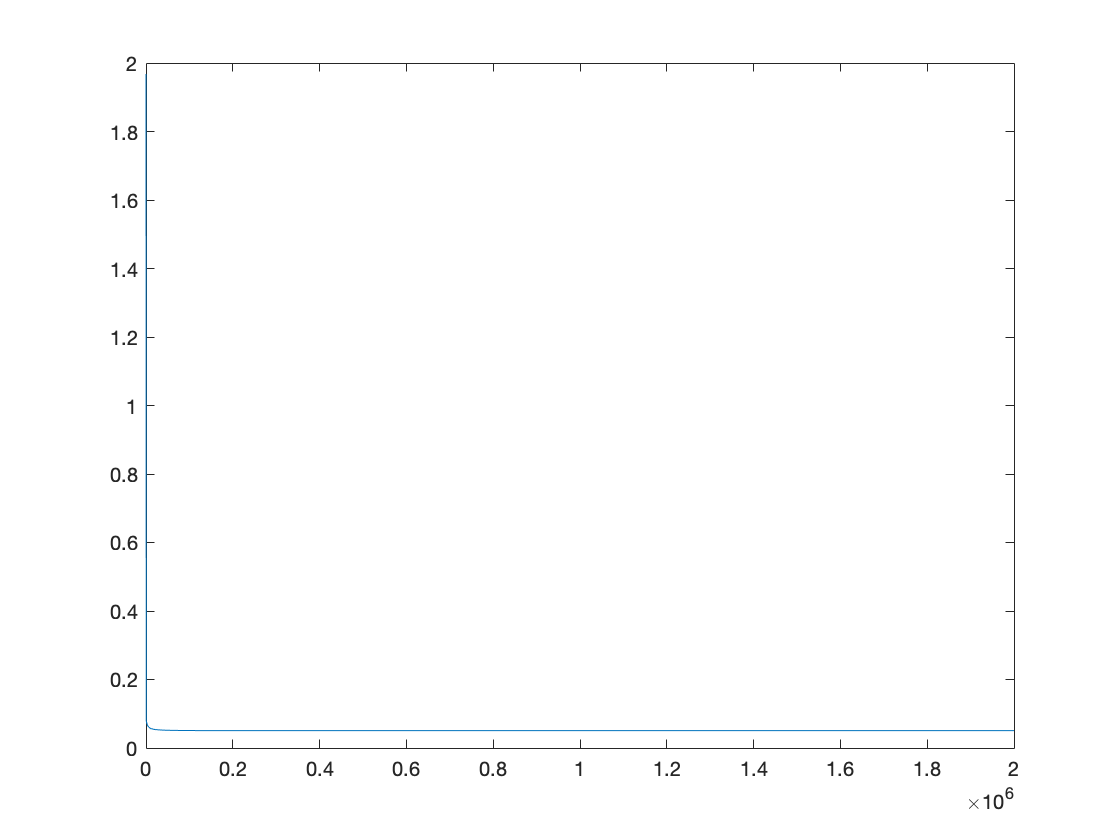
\includegraphics[width=.4\textwidth]{nndecay.png}
    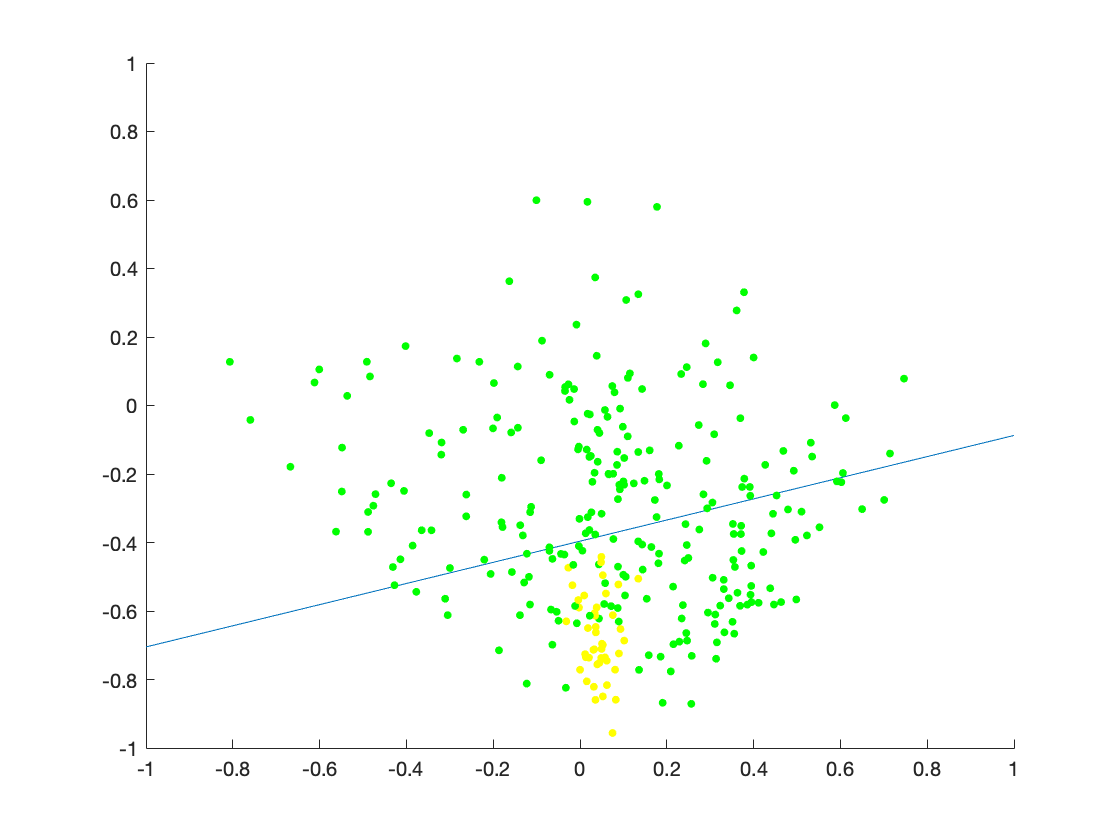
\includegraphics[width=.4\textwidth]{nndecayboundary.png}
    

  \item \textit{}



\end{enumerate}

\subsection*{Support Vector Machines.}

\begin{enumerate}[(a)]
  \item \textit{}

    For the two data points given, since there are only two points, the optimal hyperplane is 
    that which maximizes the distance from both points. If it is \textit{not} the perpendicular
    bisector, then the distance to the boundary from one point will be small compared to the
    distance from the other, and can be increased while maintaining this state. Thus the only
    solution is the hyperplane which is equidistant for both points, i.e. the perpendicular 
    bisector.

    The equation of this hyperplane is $x_1 = 0$.

  \item \textit{}

    \begin{enumerate}[i.]
      \item \textit{}

        \[ \mathbf{z}_1 =
        \begin{pmatrix} 1 \\ 0 \end{pmatrix}
          \qquad
          \vec{z}_2 = 
          \begin{pmatrix} -1 \\ 0 \end{pmatrix}
            \]

      \item \textit{}

        The optimal hyperplane in this case is the same, since the points are the same, but this
        is in Z-space:

        $$z_1 = 0$$


    \end{enumerate}

  \item \textit{}

    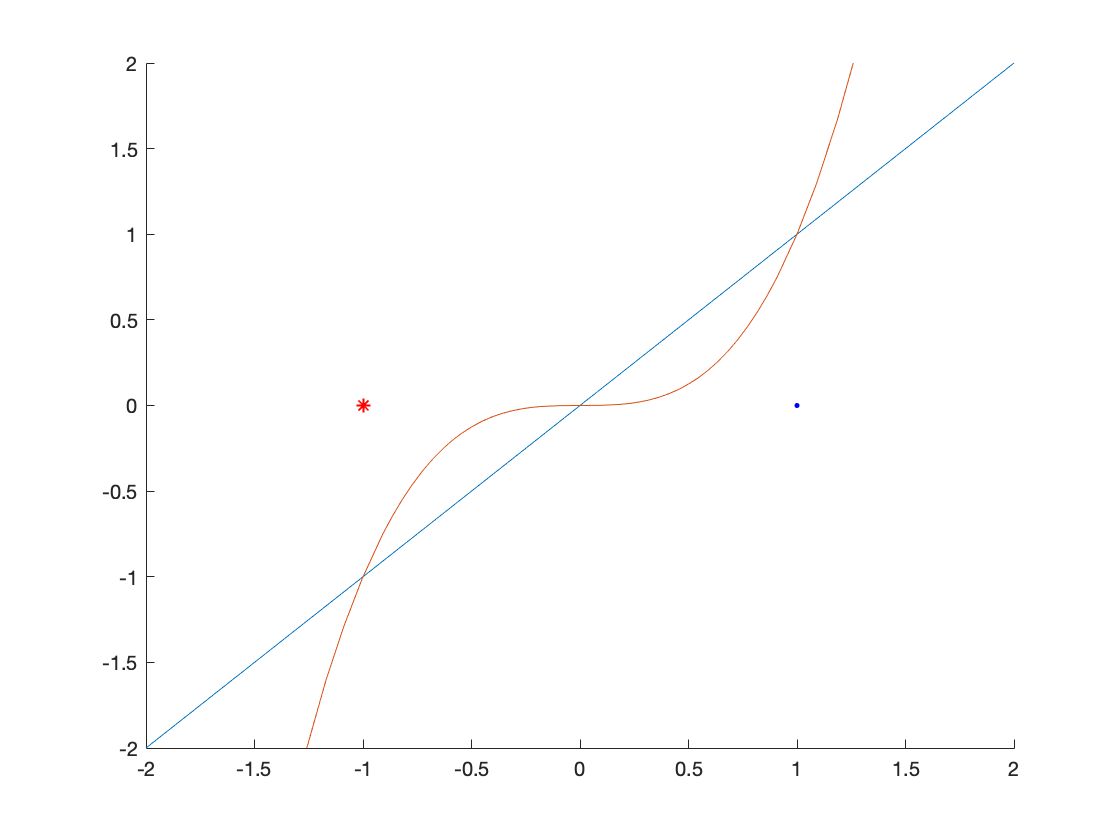
\includegraphics[width=.5\textwidth]{svmeasy.png}

  \item \textit{}

    \begin{align*}
      K(\vec{x}, \vec{y}) &= \vec{z}(\vec{x})\cdot\vec{z}(\vec{y}) \\
      &= \begin{pmatrix} x_1^3 - x_2 \\ x_1x_2 \end{pmatrix} \cdot
        \begin{pmatrix} y_1^3 - y_2 \\ y_1y_2 \end{pmatrix} \\
      &= (x_1^3 - x_2)(y_1^3 - y_2) + x_1x_2y_1y_2 \\
    \end{align*}

  \item \textit{}

    $$x_1^3 - x_2 = 0$$

\end{enumerate}


\subsection*{SVM with Digits.}

\begin{enumerate}[(a)]
  \item \textit{}

    We have C = 1 on the left and C = 5000 on the right:

    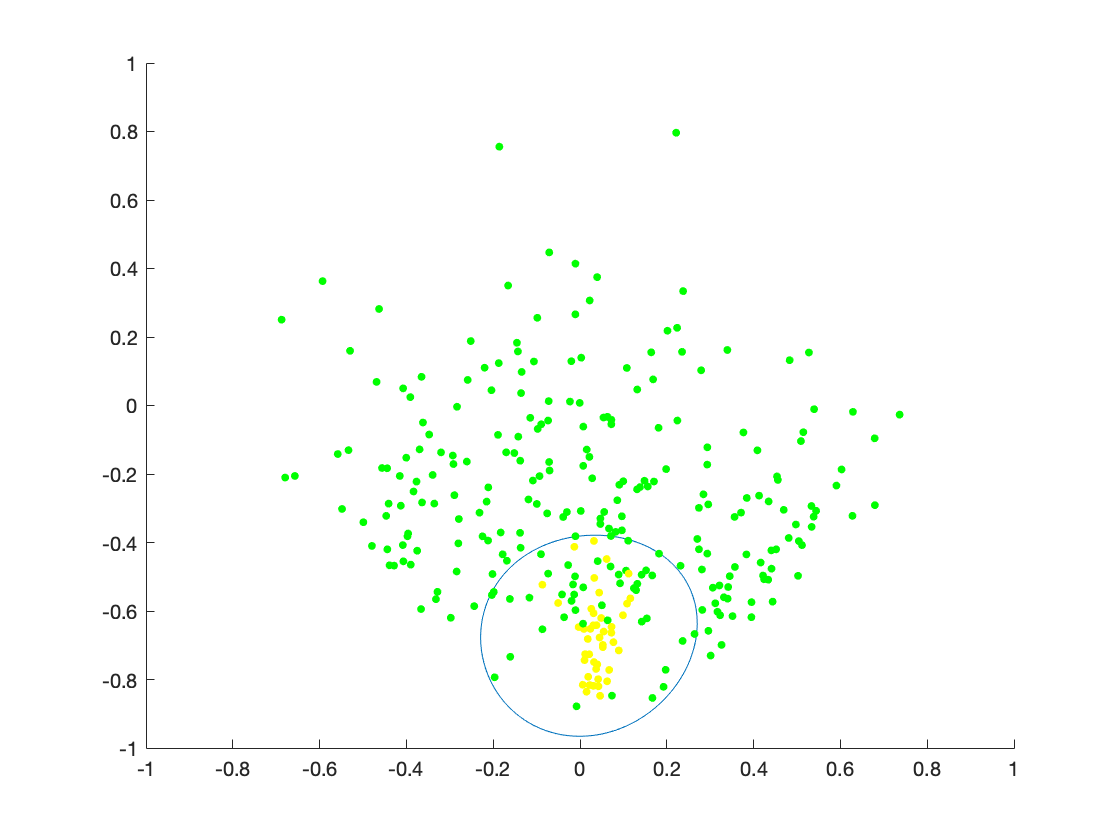
\includegraphics[width=.4\textwidth]{svmC1.png}
    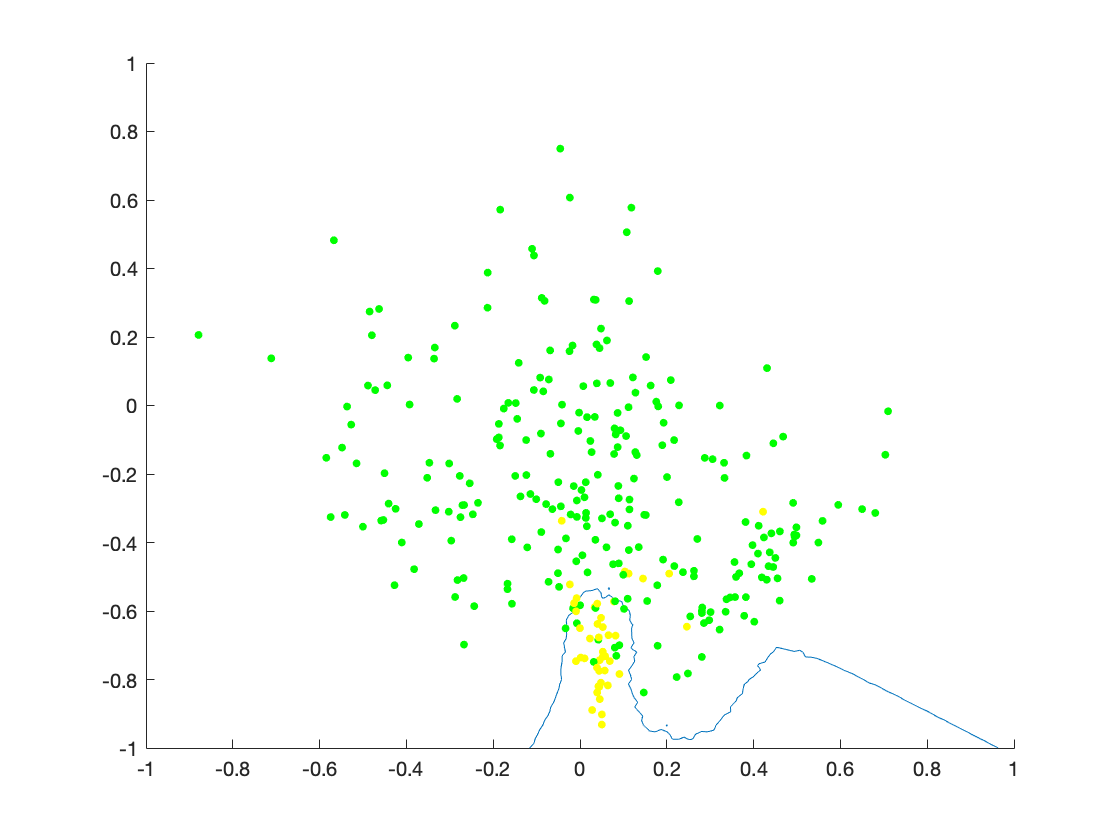
\includegraphics[width=.4\textwidth]{svmC5000.png}

    Ein is 14.33\% for C = 1, and 7\% for C = 5000.

  \item \textit{}

    The C = 1 boundary has very little "regularization" in this case, so it is underfit. On the
    other hand, C = 5000 results in overfitting, which is also undesirable and increases
    complexity of the boundary. However, the Ein is much smaller, since it aids in fitting the 
    data available better.

  \item \textit{}

    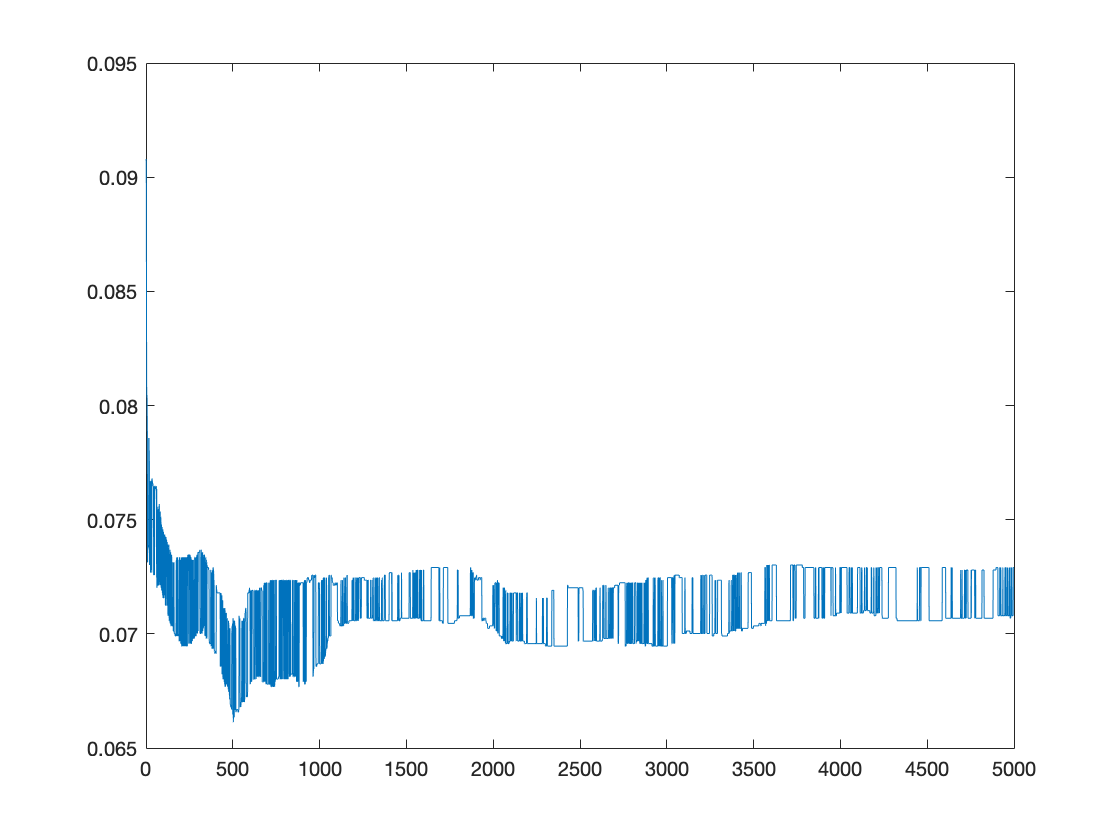
\includegraphics[width=.8\textwidth]{EcvC5000.png}

    This best error value for $1 \leq C \leq 5000$ is at $C = 493$. The resulting decision 
    boundary is

    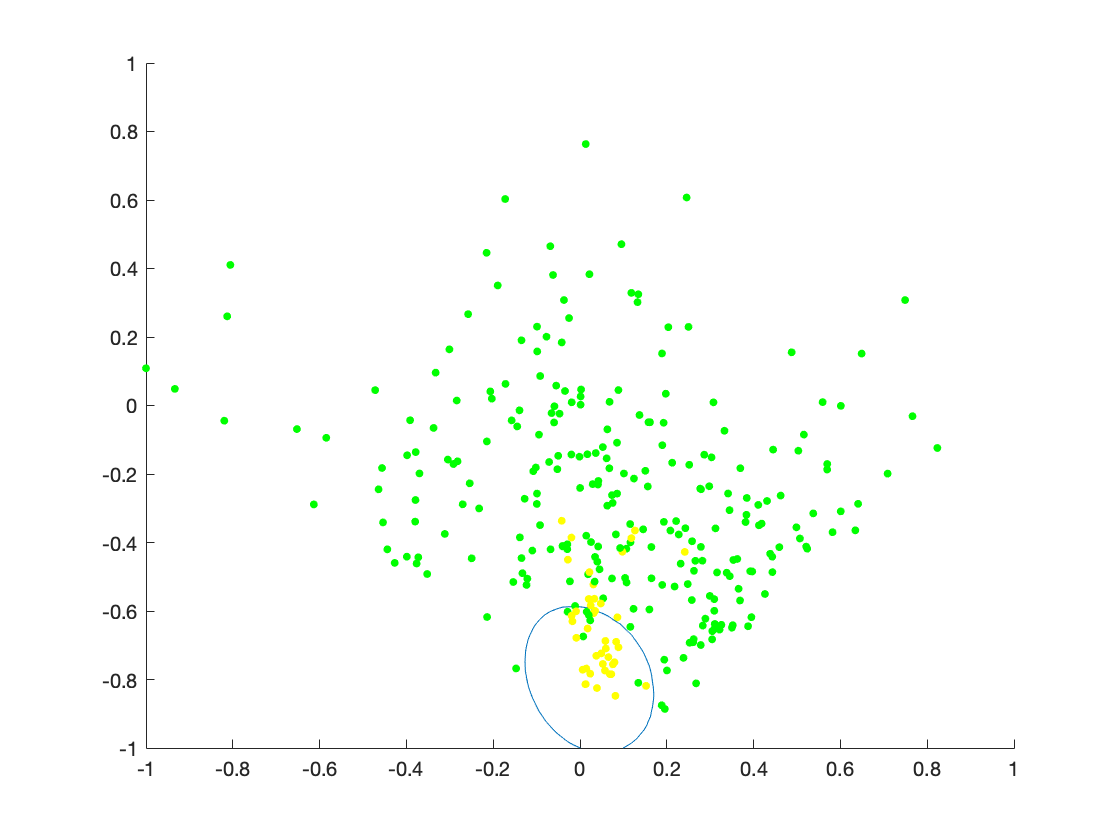
\includegraphics[width=.8\textwidth]{svmfinal.png}

    It has a test error of 6.4\%.

\end{enumerate}


\subsection*{Compare Methods.}

Overall, none of the methods used ended up being that different from each other by more than
a few tenths of a percentage point.  The approximate test error of the 3-Nearest Neighbor boundary was the
smallest of all five, at 6.1\%. Next was RBF at 6.2, SVM at 6.4, Neural Network at 6.5, and 
the 8th order Legendre transform perceptron with 6.7\% error. 

One key takeaway here is no matter how powerful the learning algorithm is, it will be handicapped
by somewhat poorly selected features that do not provide adequate separability in the data. 
This can be fixed with better defined features, or perhaps preprocessing the data so the features
are better separated. There are also preprocessing methods to select new features automatically,
and while this takes away possibly valuable information about what is going into those features,
it could help build a better classifier.

The neural network took, by far, the longest to run, at about 30 minutes for this small training
set, and given the lack of benefit in error, it makes little sense to use it versus the more
efficient RBF method. In the long run, however, when more features and more digits need to be
classified (other than just 1 and not-1), the neural network could prove more useful.

What's most important to recognize is that learning is a balancing act. Adding complexity to
the algorithms and to the data, while tempting, may actually leave you better off when it comes
to actually using the trained model. Overfitting is a significant problem. Likewise, underfitting
can be detrimental, so it's important to get the technique and the data in the right shape to 
most effectively learn. 




















\end{document}
